\documentclass[11pt,a4j]{jarticle}%jarticleを使用
\usepackage[dvipdfmx]{graphicx}%画像表示の設定
\usepackage{amsmath}%数式周りの強化
\usepackage[all, warning]{onlyamsmath}%eqnarrayを禁止
\usepackage[top=5truemm,bottom=30truemm,left=20truemm,right=20truemm]{geometry}%ページの余白を調整
\usepackage{cite}%引用を整備
\usepackage{ascmac}%screen環境による箱囲みを利用
\usepackage{url}%urlを成形する
\usepackage{here}
\usepackage{listings,jvlisting} %日本語のコメントアウトをする場合jvlisting(もしくはjlisting)が必要
%ここからソースコードの表示に関する設定
\lstset{
  basicstyle={\ttfamily},
  identifierstyle={\small},
  commentstyle={\smallitshape},
  keywordstyle={\small\bfseries},
  ndkeywordstyle={\small},
  stringstyle={\small\ttfamily},
  frame={tb},
  breaklines=true,
  columns=[l]{fullflexible},
  numbers=left,
  xrightmargin=0zw,
  xleftmargin=3zw,
  numberstyle={\scriptsize},
  stepnumber=1,
  numbersep=1zw,
  lineskip=-0.5ex
}
%ここまで表示に関する設定
\begin{document}

\section*{演習2}
\begin{figure}[H]
  \centering
  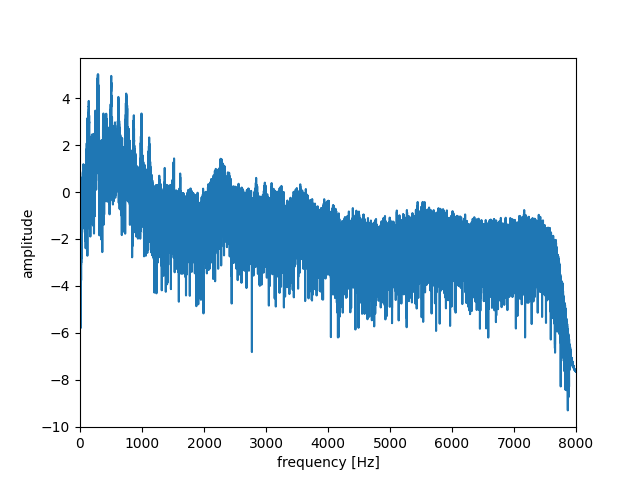
\includegraphics[width=120mm]{img/aiueo-plot-spectrum-whole.png}
  \caption{aiueo.wavの波形とスペクトル}
\end{figure}

\begin{figure}[H]
  \centering
  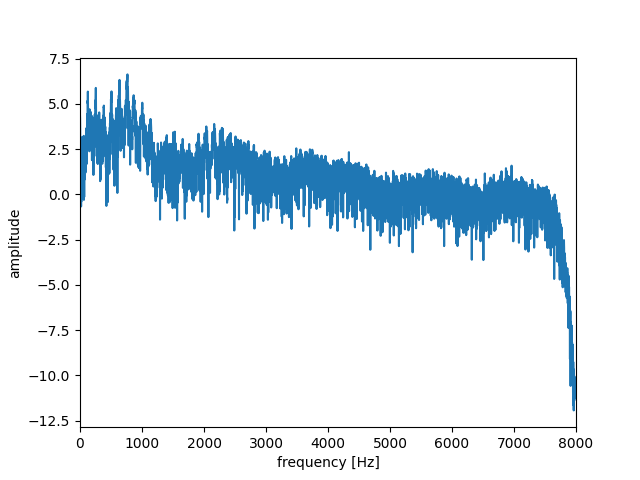
\includegraphics[width=120mm]{img/a-plot-spectrum-whole.png}
  \caption{a.wavの波形とスペクトル}
\end{figure}

\begin{figure}[H]
  \centering
  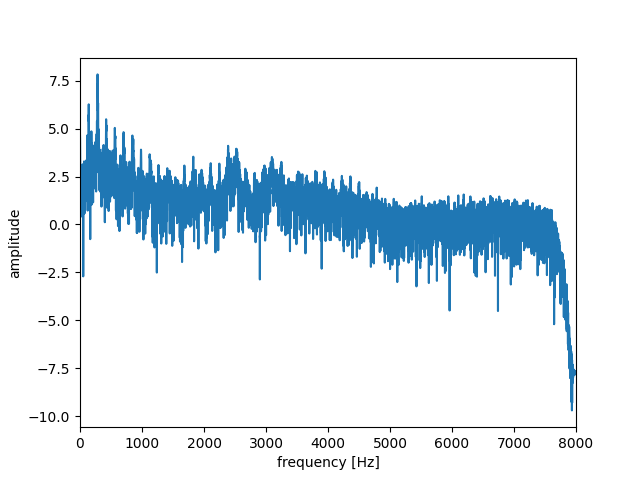
\includegraphics[width=120mm]{img/i-plot-spectrum-whole.png}
  \caption{i.wavの波形とスペクトル}
\end{figure}

\begin{figure}[H]
  \centering
  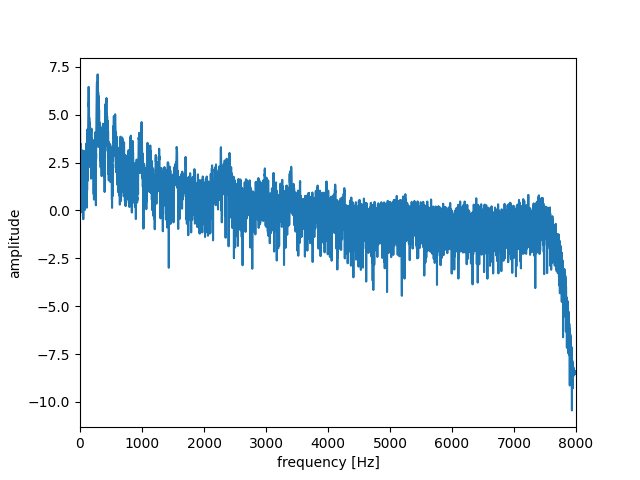
\includegraphics[width=120mm]{img/u-plot-spectrum-whole.png}
  \caption{u.wavの波形とスペクトル}
\end{figure}
\begin{figure}[H]
  \centering
  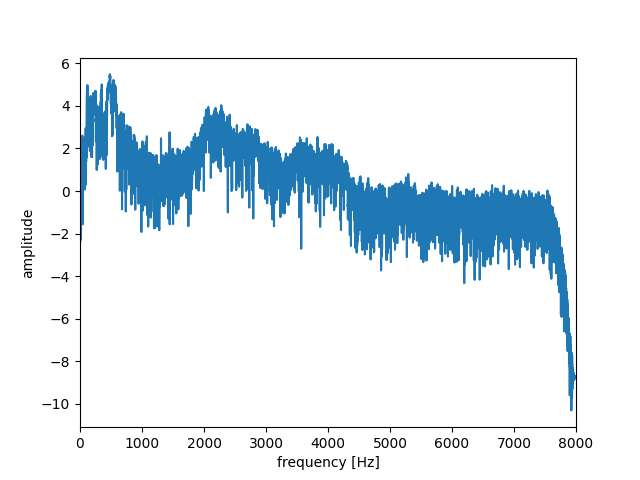
\includegraphics[width=120mm]{img/e-plot-spectrum-whole.png}
  \caption{e.wavの波形とスペクトル}
\end{figure}

\begin{figure}[H]
  \centering
  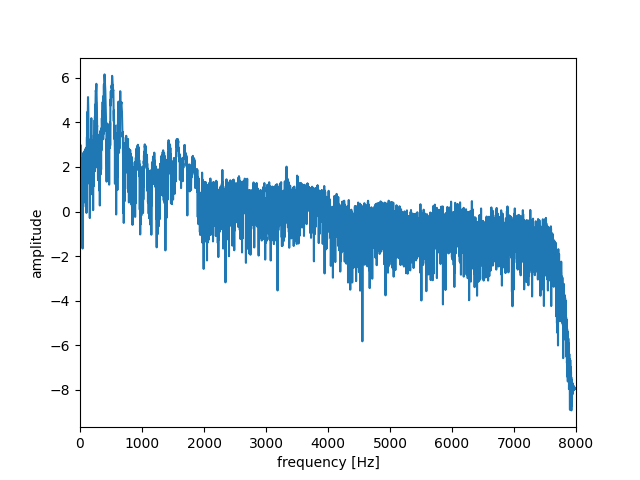
\includegraphics[width=120mm]{img/o-plot-spectrum-whole.png}
  \caption{o.wavの波形とスペクトル}
\end{figure}

\section*{演習3}
実数入力に対する1次元離散フーリエ変換を計算するするライブラリ.
高速フーリエ変換(FFT)によって、実数値配列の1次元n点離散フーリエ変換(DFT)を計算する.
入力は実数値配列で、出力は複素数値配列である.
入力には他にも $n$(使用する入力内の変換軸に沿ったポイントの数, optional),axis(変換を行う軸, optional) を指定できる.

※純粋な実数入力に対して DFT を計算すると、出力はエルミート対称($その成分は任意の添字 i, j について (i, j)成分は (j, i)成分の複素共役と等しい.$)になる.
つまり、負の周波数項は対応する正の周波数項の複素共役にすぎない.
したがって負の周波数項は冗長になるのでRFFTでは負の周波数項を計算しない.
その結果、出力の軸の長さは $\lfloor n/2 \rfloor+ 1
$になる.
\section*{演習4}
\subsection*{バタフライ演算}
\paragraph*{DFTについて}
そもそも、DFTでは$N$点の実変数 $f(0),f(1), ... ,f(N-1)$を離散フーリエ変数 $F(0),F(1), ... ,F(N-1)$に変換するために
$N$次正方行列であるDFT行列を掛け合わせているのだった.
この計算では,$O(N^2)$となる.この計算量を軽減するために、高速フーリエ変換(FFT)が考案された. 
\paragraph*{FFTの計算量}
上述の通りDFTでは計算量が多いので、バタフライ演算を用いて計算量を減らしている.
\subsection*{FFTの実践(手計算)}
input $= (1,0,3,2,4,0,2,0)^T $
\begin{align}
(略)
\end{align}
以下で計算が正しいことを検証する.
\begin{lstlisting}[caption=FFTの実践(numpy篇),label=prog1]
>>> import numpy as np
>>> np.fft.fft([1,0,3,2,4,0,2,0])
array([12.        +0.j        , -4.41421356-2.41421356j,
      0.        +2.j        , -1.58578644-0.41421356j,
      8.        +0.j        , -1.58578644+0.41421356j,
      0.        -2.j        , -4.41421356+2.41421356j])
\end{lstlisting}

\end{document}
